\documentclass[a4paper,11pt]{jsbook}

% 目次リンク
\usepackage[dvipdfmx]{hyperref}
\usepackage{pxjahyper}
% 数式
\usepackage{amsmath,amsfonts}
\usepackage{bm}
% 画像
\usepackage[dvipdfmx]{graphicx}
\usepackage[dvipdfmx]{color}

\begin{document}

\title{Splatoon}
\author{さとうあずき}
\date{\today}
\maketitle
\tableofcontents


\chapter{最初の一歩}
\section{コントローラーの操作}
ZRでメインウェポンで攻撃ができる。Lスティックでキャラクターを移動できる。
\begin{figure}[h]
  \begin{center}
    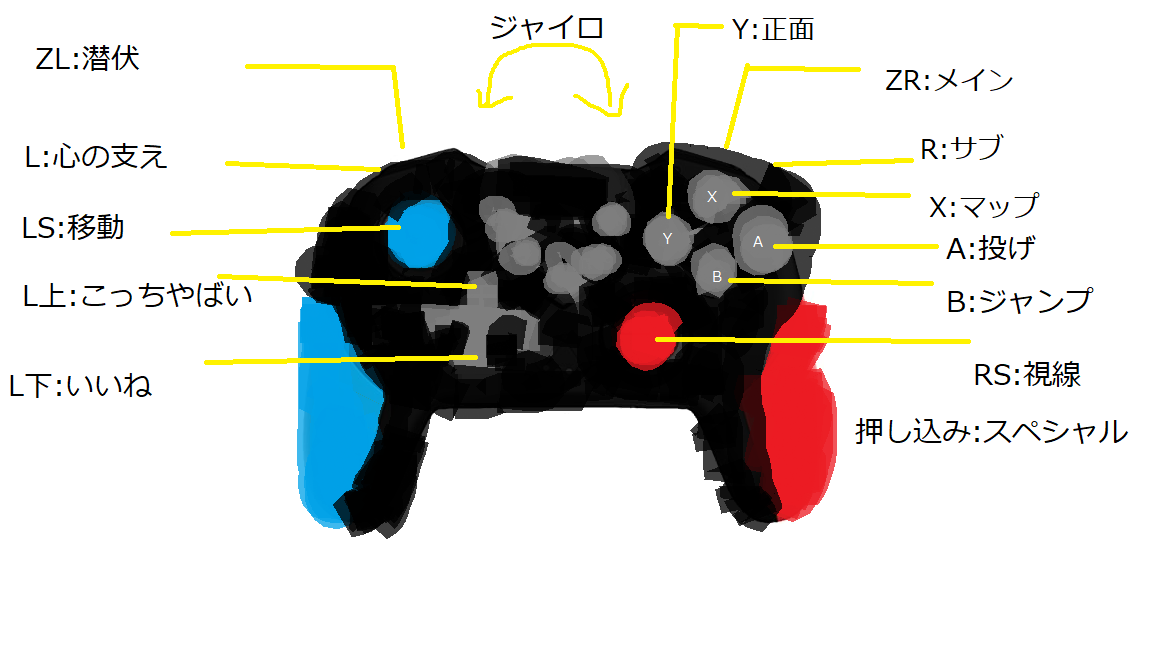
\includegraphics[width=10cm]{resoource/Controller_button.png}
  \end{center}
\end{figure}

試合画面
上に味方と敵のイカマークがある。敵味方の存命がわかる。
右上にスペシャルゲージがある。たまったら、Rスティック押し込みでスペシャルウェポンが使える。
画面中心にレティクルがある。この中に敵を入れてメインウェポンで狙える。ZRでメインウェポンで倒せる。
\begin{figure}[h]
  \begin{center}
    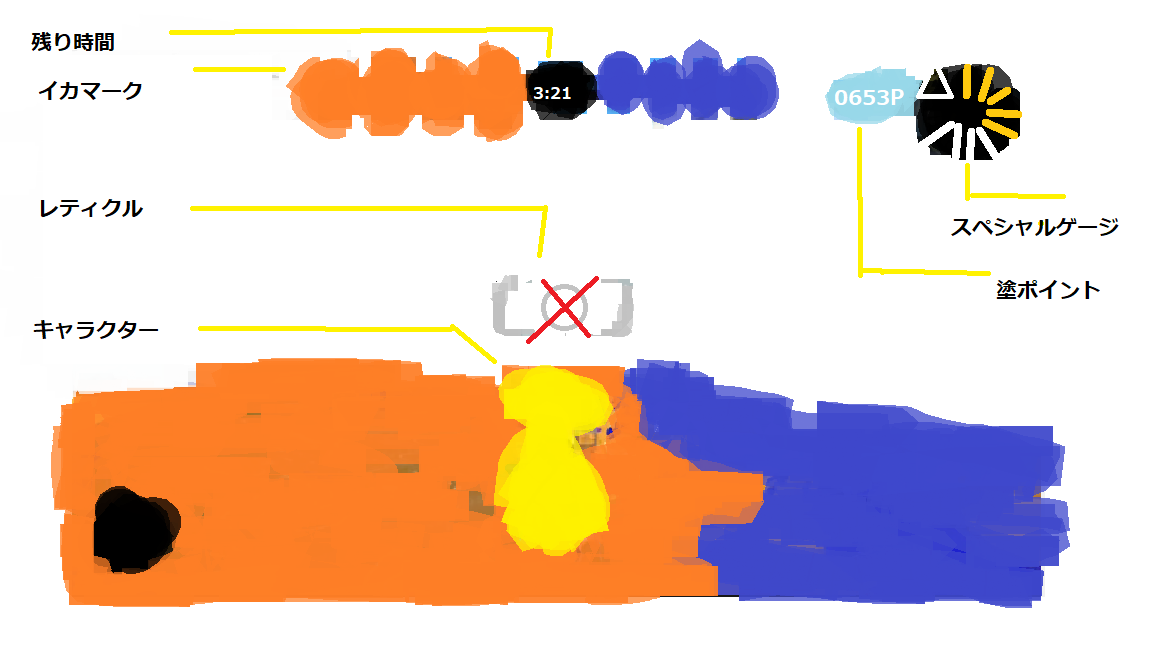
\includegraphics[width=10cm]{resoource/gamescreenframe.png}
  \end{center}
\end{figure}
\section{敵の倒し方}
\subsection{敵との位置関係}
同じ射程の武器同士ではどう戦うべきか。
同じ射程で打ち合い始めて相手に弾が当たらなかったとき移動するべきだろうか
簡単に2次元で敵と対面した時の状況を考える。
\begin{figure}[h]
  \begin{center}
    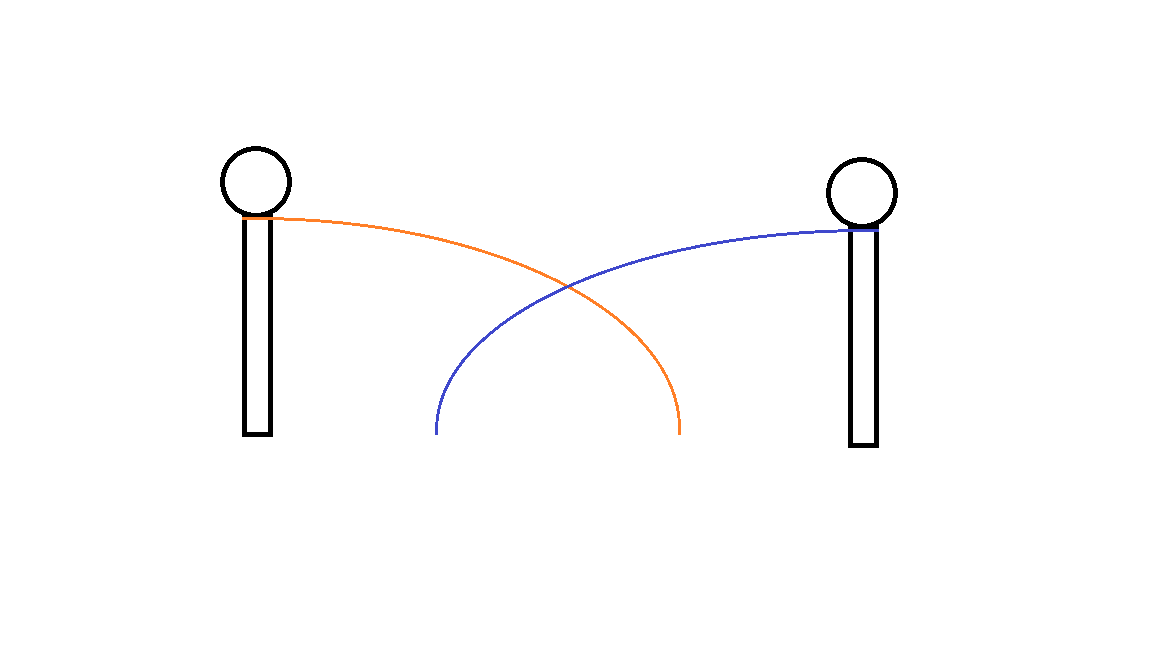
\includegraphics[width=10cm]{resoource/samerange.png}
  \end{center}
\end{figure}

同じ射程で打ち合い始めて相手に弾が当たらなかったとき近づくとどうなるか。
実は、打ち合いに負けてしまう。
自分が近づくと、相手がすでに撃っている弾に自分からあたりに行くことになる。
一方で、自分の弾は近づいて撃ち始めた所で相手にはまだ届いていない。
その結果、先にダメージがたまるのは自分になってしまう。
\begin{figure}[h]
  \begin{center}
    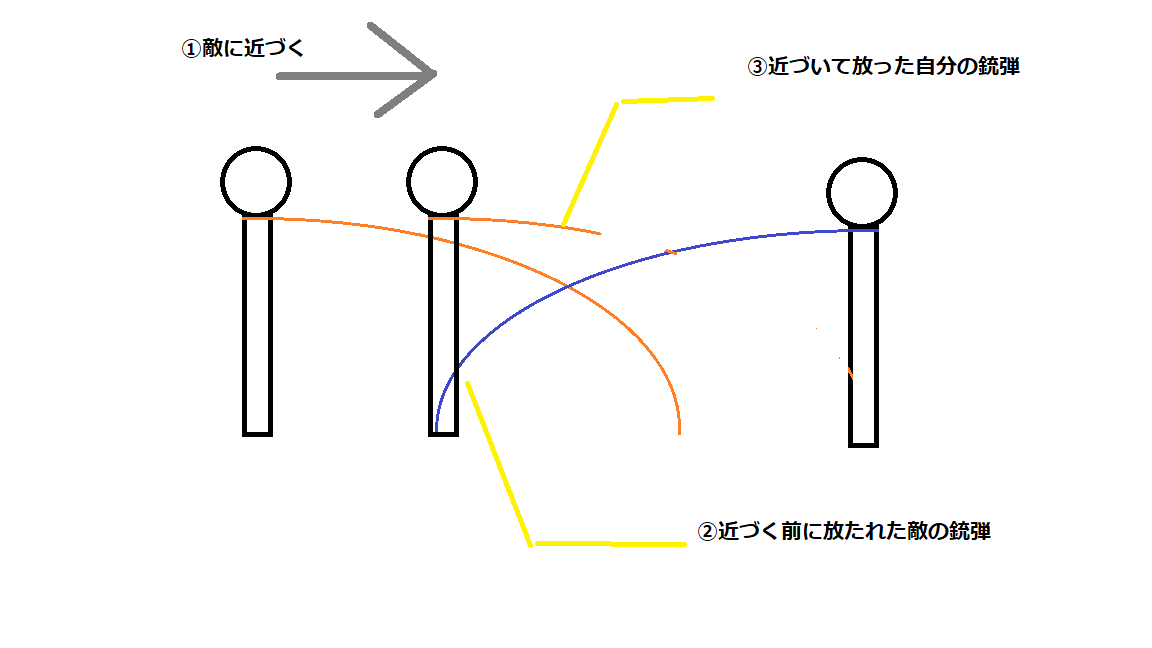
\includegraphics[width=10cm]{resoource/samerange_attacking.png}
  \end{center}
\end{figure}

相手が自分より長射程の武器場合で、打ち合い始めて相手に弾が当たらなかったとき移動するべきだろうか
同様に簡単に2次元で考える。
先ほどと同じように、自分が近づくと、相手がすでに撃っている弾に自分からあたりに行くことになる。
一方で、自分の弾は近づいて撃ち始めた所であっても相手に届くことにはならないだろう。
その結果、先にダメージがたまるのは自分になってしまう。
\begin{figure}[h]
  \begin{center}
    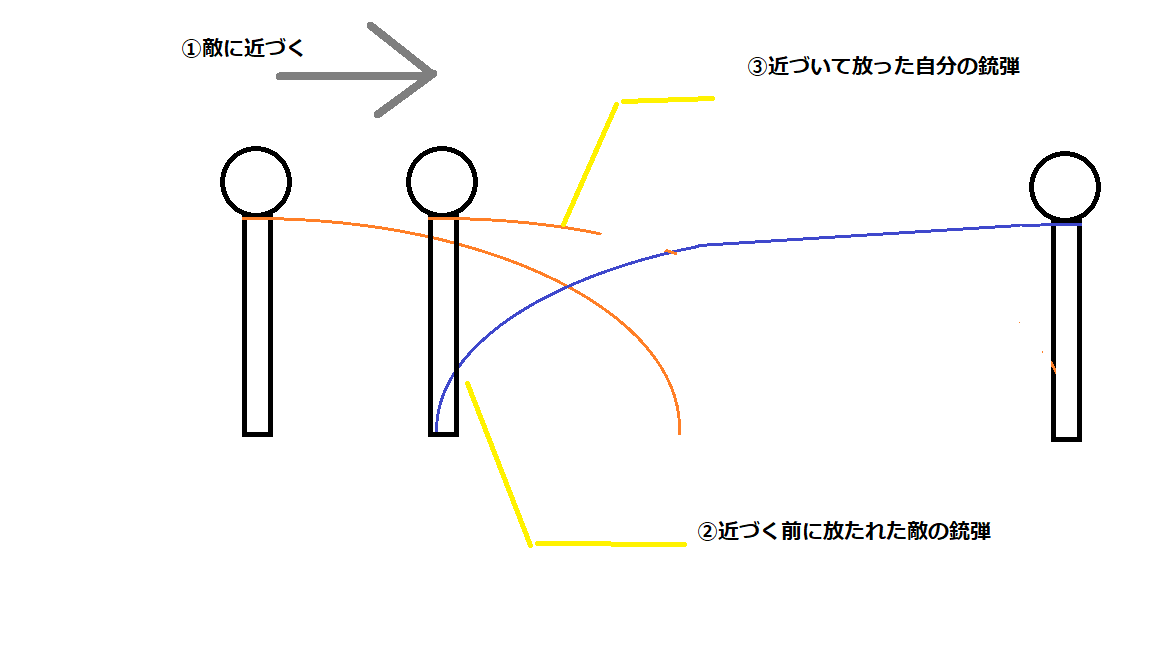
\includegraphics[width=10cm]{resoource/long_range_attacking.png}
  \end{center}
\end{figure}


相手が自分より短射程の武器場合で、打ち合い始めて相手に弾が当たらなかったとき移動するべきだろうか
同様に簡単に2次元で考える。
先ほどと同じように、自分が近づくと、自分の弾が先に相手に当たる所がある。
その結果、先にダメージがたまるのは敵になる。
しかし、自分の弾が先に相手に当たる所よりさらに近づくと、相手がすでに撃っている弾に自分からあたりに行くことになる。

\begin{figure}[h]
  \begin{center}
    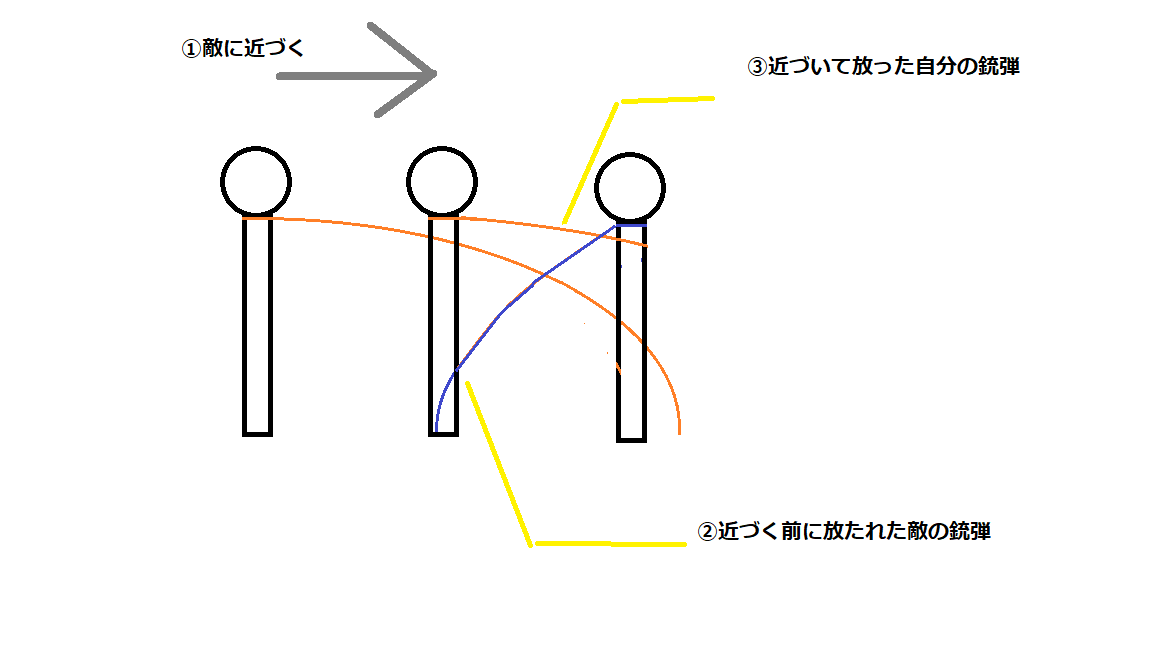
\includegraphics[width=10cm]{resoource/short_range_attacking.png}
  \end{center}
\end{figure}

以上から、2次元平面内で敵に近づくという戦術はよくない。
自分の射程以上に長い相手には近づくとやられる。
自分が相手より射程が長いときは、相手の射撃が当たらない位置まで近づくことはできるが、それ以上近づくと負ける要素が出てくる。
もちろん、実際のゲームは3次元で行われる。武器も単位時間あたりの弾の数が異なるし、弾当たりのダメージも異なる。プレイヤーは逃げ回るし、狙う対象ががプレイヤーとも限らない。
このような要素から勝負の駆け引きは発生するが、基本的に射程が届かない相手を倒すことはできない。自分の射程と相手の射程を念頭に勝負を始めよう。

相手を倒そうと意気込むだけで相手に近づくのは悪手であることが多い。\footnote{諸。敵に何度もやられようが正面から何度も突っ込みまくるプレイヤー。猪の対義語に芋がある。}
諸突猛進するプレイヤーが悪いとは思わない。ただし、プレイヤーが持つ戦術が猪しかないというのは心もとない。
じゃんけんでグーしか出さないという戦術を進んで行う人はいないだろう。

\subsubsection{射程の暴力}
敵の倒し方からわかるように、長い射程のほうが勝負を有利に進められる。長い射程であれば敵から攻撃を受けることなく一方的に敵を蹂躙し、試合に勝つことができてしまう。
これを射程の暴力と呼ぶ人もいる。
シューティングゲームでは、長射程武器を持つ敵をどうやって倒すかがとても大事になってくる。

\subsection{敵との距離の詰め方}
敵と対面した位置関係について2次元的に考えた時には近づくという方法は基本的に不利になるという説明をしていた。
しかし、自分の武器の射程範囲に敵がいなければ敵を打ち倒すことはできない。

一方で、3次元空間において敵と対面していない場合ではお互いの距離を近づけてよいだろうか?
答えは、「はい」となる。
この小節では敵との距離をどう詰めるかについて考えてみる。
\subsubsection{敵に近づく}
敵を見つけて近づくのは二次元的に対面していた場合は不利であるが、敵と対面していない場合はそうではない。
敵はいつも自分を見ているわけではなく、そのため敵が自分と対面していない時が距離を詰めるチャンスである。
ここでは敵に近づくためにどうやって敵に自分以外に対面してもらうかを考える。
一番簡単なケースは、注目している敵が味方と対面している場合だ。これは自分と味方と敵を頂点に取ると三角形になる。
よく球技ではこの三角形を意識してチーム連携を取るが、それと全く同じである。
このように敵が別のものに対面せざるを得ないモノはいくつかある。
例えば、一撃で倒せるサブウェポンやスペシャルウェポンである。敵は一撃でやられるのを回避するために、そのウェポンに対面あるいは視野に入れざるを得ない。
他には試合に勝つために必要なルール関与オブジェクトである。スプラトゥーンのガチマッチであれば、エリアやホコ、ヤグラ、そしアサリになる。
技術や機会で限られるケースに、たとえば自分の残像や敵が潜伏している場所にも対面させることができる。

\subsubsection{敵が近づく}
対面していない敵が自分のところに近づいてくるケースはいくつかある。
よくあるのは通路の近くで隠れることで敵は近づいてくる。
ステージの角であったりモノの影にひそめたりすることで、敵が攻めてくることはよくある。
道に伏せる、高い位置を取るといった、地平線に自分の身が映らない場所というのも、相手は気が付かないことが多い。
特にスプラトゥーンでは、地面に塗られた自分のインクの中に身をひそめることができる。

\subsection{敵を撃つやり方}
さて、ようやく自分のメインウェポンの射程圏内に敵が入ってきた。ここで敵を倒すには自分の銃で弾を当てよう。
スプラトゥーンに限らずシューティングゲームであれば画面の真ん中に向かって弾が飛んでいくだろう。
標準を自動補正してくれるゲームもあるが、スプラトゥーンでは補正をしてくれない。

スプラトゥーンでは画面中央に射撃範囲とレティクルがある。弾は限らず射撃範囲内に飛び出す。
レティクルで当たり判定があれば弾が届くが、当たり判定がなければおよそ弾は届かない。

\chapter{ガチマッチで勝つ}
本当はガチマッチで勝つ方法はもっと後に記述したかった。
\section{ガチエリア}
\subsection{カウントを進める}
マッチルールオブジェクトと前線、戦線
マッチルールオブジェクトはエリアになり、エリアはステージ中心に存在する。
オブジェクト付近に敵を近づけさせないために、前線はステージ中心のエリアより敵陣側
前線と敵陣リスポーンの間に戦線が発生する
武器の役割や敵のポジションといった環境によるが、基本的に自身のカウントが進んでいるときにエリアより自陣側にポジションを取るメリットはない。
敵陣側では相手がエリアに来るのに時間がかかるようなポジショニングをしよう。たとえば、浮いた敵を倒せる壁影や、高所といった相手に不利になる場所に陣をとろう。
ほかにも敵陣で自陣の塗りを広げておくだけでもよい。
エリア付近に残る場合、スペシャルゲージをためて置いたり、敵陣に進んだ味方のフォローに入れるようにしよう。

\subsection{カウントを奪う}
マッチルールオブジェクトと前線、戦線
マッチルールオブジェクトはエリアになり、エリアはステージ中心に存在する。
オブジェクト付近に近づくために、前線がステージ中心にある
戦線と自陣リスポーンの間に前線が発生する
基本的に敵のカウントが進んでいるときにエリアより敵陣側にポジションを取るメリットはない。
敵のカウントが進んでいるとき、基本的に戦線はエリアより自陣側になるはずである。
もし戦線がエリア付近であれば人数有利になったタイミングでエリアをすぐに塗り返せるので焦る必要はない。
逆に戦線がエリアより自陣にある場合、戦線をエリアに押し上げよう。

\section{ガチヤグラ}
\subsection{カウントを進める}
マッチルールオブジェクトはヤグラになり、ヤグラは決まった進路に沿って敵陣に移動する。カウントはその最大移動距離と連動する。
進路には関門があり、関門にヤグラが到達すると一定のカウントを進めるまで同じ位置にあり続ける。
オブジェクト付近に敵を近づけさせないために、前線はヤグラより敵陣側。ヤグラと敵陣リスポーンの間に戦線が発生する。

\subsection{カウントを奪う}
マッチルールオブジェクトはヤグラになり、ヤグラは決まった進路に沿って自陣に移動する。
進路には関門があり、関門にヤグラが到達すると一定のカウントを進めるまで同じ位置にあり続ける。
ヤグラを自陣に近づけさせないために、ヤグラと自陣陣リスポーンの間に前線が発生する。
戦線線はヤグラ付近。基本はヤグラを止めるのは関門で行う。動いている敵を狙い続けるは難しい。
ほかにも決まった位置にヤグラが来る、つまり決まった場所に敵がいることになるので、事前に有利なポジションに配置つける。
スペシャルウェポンを関門にやってきたタイミングで使うとよい。







\section{ガチホコ}
\subsection{カウントを進める}
マッチルールオブジェクトはホコになり、ホコを持つプレイヤーは自由に進路を選べて敵陣に移動する。
ホコはゴールまでの距離によってカウントを進めることができる。壁のぼりではカウントは進めない。

オブジェクト付近に敵を近づけさせないために、前線はホコより敵陣側。ホコと敵陣リスポーンの間に戦線が発生する。


\subsection{カウントを奪う}
マッチルールオブジェクトはホコになり、ホコを持つ敵プレイヤーは自由に進路を選べて自陣に移動する。
ホコはゴールまでの距離によってカウントを進められる。

自陣付近にホコを近づけさせないために、戦線はホコ付近やその敵陣側。ホコと自陣リスポーンの間に前線が発生する。

\section{ガチアサリ}
\subsection{カウントを進める}
マッチルールオブジェクトはアサリになり、ガチアサリを持つプレイヤーは自由に進路を選べて敵陣に移動する。
ゴールにガチアサリやアサリを投入するとカウントを進めることができる。

ゴールにガチアサリやアサリを投入するために、
前線はゴールより自陣側。ゴールと敵陣リスポーンの間に戦線が発生する。

\subsection{カウントを奪う}
マッチルールオブジェクトはアサリになり、ガチアサリを持つプレイヤーは自由に進路を選べて敵陣に移動する。
ゴールにガチアサリやアサリを投入されるとカウントを進められる。

ゴールにガチアサリやアサリを投入させないために、
前線はゴールより自陣側。ゴールと敵陣側に戦線が発生する。


\chapter{初めに}
\section{Splatoon}
\subsection{ゲームが目指しているところ}
人は目が覚めたらご飯を食べ、トイレに行き、将来に向けてあくせくと働き、そして寝る。
最適化された生活の中には喜怒哀楽もなく、ただ平然と人生を消費していき、死ぬ。
最適化された生活から脱却するような無駄な行為である。
しかし、人生において無駄な行為こそ、人生を謳歌するための唯一の手段である。
人生においてゲームは必要ない。だからこそゲームの中での一喜一憂は我々の生活を豊かにし、そして生まれた意味になる。

\subsection{Splatoon3とは}
Splatoon3は2022年9月8日に任天堂から発売開始され、発売3日間で国内販売本数345万本を記録した大人気ゲームソフトである。
このゲームはイカやタコが4対4のチームを組み、インクを垂らしながら陣地を奪ったりルールに基づいてポイントを稼いだりして勝敗を決める、新感覚のシューティングゲームである。
老若男女問わず楽しめるもので初心者からプロもプレイし、このゲームを通して世界中のプレイヤーはゲームのランキングを競いあっている。

\subsection{Splatoonへの憤り}
Splatoonは大変面白いゲームであり、世界中から愛されている。
素晴らしいプレイがあれば喜び、強い敵に打ち負かされて悲しみ、このゲームを通して我々は充実した時間を過ごすことができるだろう。
しかし、Splatoonをこよなく愛するプレイヤーの中にはどうやらただただストレスをうけ、さらにそのプレイヤーの罵声や怒号によって周りの人間を不愉快にさせ、何のためにゲームをやっているのかわからなくなっている人がいるようだ。
私はそんな人たちが少しでも充実したゲーム人生を過ごしてもらうと、筆を執ることにした。


\section{ゲームを楽しむ}
本当は最初に敵を倒す方法についてまとめはしたくなかった。
ゲームという時間を忘れてゲーム目標を達成する快感や、ゲームの世界観を満喫することに集中してほしいと思っていた。
ただ、この文章を読んでほしい相手は、スプラトゥーンの世界を隅から隅まで楽しむことより、まずは目の前の敵を倒したいという欲望にとらわれていた。
そのため、折角始めてくれたゲームなのに、私の伝えたいことを一方的に説明するのではなく目の前の敵を倒す、一般的な考え方について記述した。
しかしそれでもやはり、お金と時間を使って始めたゲームを通して、自分の生活をより良いものにしてほしいと切に願う。
決して対人ゲームに負けてストレスを抱えたり、まして周りの人間にストレスを与える存在になってほしくはないと思う。
\subsection{勝負に勝つ}


\subsection{試合に勝つ}





\chapter{試合を優位に進める}
\section{大局的人数有利}
\subsection{通信障害}
\subsection{イカマーク}
\subsection{マッチルールオブジェクト}
マッチルールオブジェクトを味方と考える。→三角関係

\section{局所的人数有利}
\subsection{三角関係}
自分と相手と何か
味方
ルール関与オブジェクト
自分の残像



\subsection{戦線}
敵と味方が打ち合っている境界線
\begin{figure}[h]
  \begin{center}
    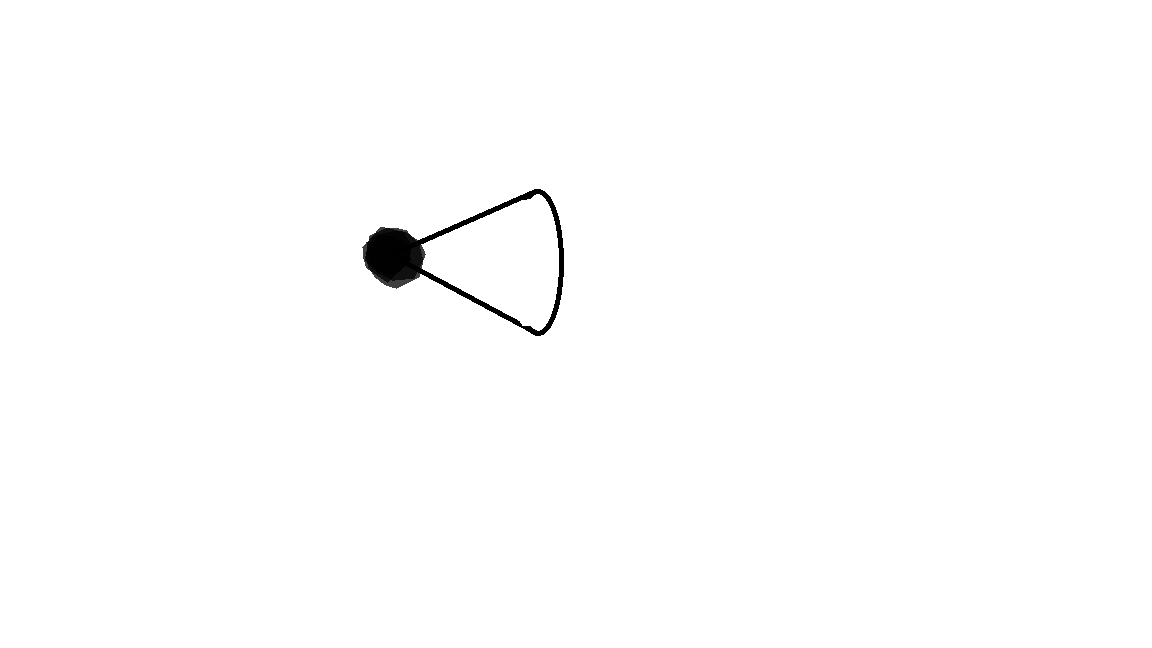
\includegraphics[width=10cm]{resoource/player.png}
  \end{center}
\end{figure}

\subsection{前線}
戦線にヘルプに入れる位置で自陣のリスボーンに一番近い位置

\section{地形有利}
\subsection{高所}
相手の位置がわかる、自分の位置は相手はわからない

\subsection{オブジェクト}
\section{チーム構成有利}
\subsection{スペシャルウェポン有利}
打開
射程
\subsection{サブウェポン有利}
打開
射程
\subsection{メインウェポン有利}
打開
射程
\subsection{ギア有利}
打開
射程

\chapter{勝負を優位に進める}
\section{メインウェポン}
\subsection{射程と索敵}
\subsection{射程とキル}
\section{サブウェポン}
\subsection{索敵}
\section{スペシャルウェポン}
\section{イカ状態とヒト状態}
\subsection{当たり判定}
ヒト状態とイカ状態
右打ち
\subsection{インク回復}
\subsection{移動速度}
\subsection{インク潜伏}
\section{マップ}
\section{キャラクター移動}
\subsection{風神雷神}
\section{スーパージャンプ}
\section{ジャンプ}
\section{やられたとカモンとナイス}
\section{カメラリセット}


\chapter{謝辞}

\appendix
\chapter{A}



\begin{thebibliography}{2}

\bibitem{K.miyuki}K.miyuki (private communication)
\end{thebibliography}

\thispagestyle{empty}
\vspace*{\stretch{1}}
\begin{flushright}
\begin{minipage}{0.5\hsize}
\begin{description}
  \item{著者:}さとうとーま
  \item{挿絵:}さとうとーま
  \item{発行:}\date{\today}
  % \item{印刷:}POPLS (\verb|http://www.inv.co.jp/~popls/|)
\end{description}
\end{minipage}
\end{flushright}

\end{document}











